%\addcontentsline{toc}{chapter}{Introduction}
\chapter{Introduction}
Mathematical modeling and scientific computing has become an inseparable part of engineering and science, thanks to advances in computational science and technology. Models expressed as partial differential equations (PDEs) can be found in a wide range of disciplines from social sciences, biology, cosmology, modern and classical physics, and engineering to industrial applications. The overwhelming success of such models for approximately describing nature has encouraged the development of complex mathematical models in order to attain higher accuracy in representing physical phenomena. The complexity of many modern applications, however, is computationally prohibitive with classical approaches. The curse of dimensionality for multi-dimensional parameter sets, i.e. the exponential growth in the computational costs for problems in higher dimensions, is an example of a computational inefficiency that inhibits progress.

Reduced order modeling (ROM), as opposed to high-fidelity modeling, has emerged as a successful attempt to reduce the intrinsic computational inefficiencies of modern complex models \cite{hesthaven2015certified,quarteroni2015reduced,doi:10.1137/1.9781611974829,doi:10.1137/1.9780898718713}. ROM aims to accurately represent a high-dimensional model with a few degrees of freedom, by exploiting empirical or physical structure in data. As a result of confining the model to only these degrees of freedom, the computational costs can be substantially reduced. Although these methods do not eliminate the need for high-fidelity modeling, they significantly accelerate the evaluation of outputs of interest when the repeated evaluation of the high-fidelity model is required \cite{hesthaven2015certified}.

%Reduced basis (RB) methods, are a class of techniques for ROM, which restricts the high-fidelity model to a subspace with a, relatively, low dimension. Representing the high-fidelity model in this subspace, using a projection operator, reduces the system size of the system of algebraic equations that describe the model. 

The recognition of patterns in data makes ROM comparable with machine learning techniques, e.g. in computer science and statistics developed during the past decades \cite{machinelearning}. However, the deterministic nature of PDEs, Combined with the control in the choice of data generation process, gives ROM a distinct take. 

This difference between ROM and conventional machine learning techniques becomes more apparent with time-dependent problems. Time-symmetries of high-fidelity models are lost in the assembly of data, which sometimes, result in an ill-represented ROM \cite{doi:10.1137/1.9780898718713}. Although this inaccuracy in the representation is less evident for parabolic PDEs, the development of ROMs for hyperbolic PDEs, where symmetries are a fundamental feature, remains a challenge \cite{doi:10.1137/17M1111991,kalashnikova2014stabilization,farhat2015structure,doi:10.1137/110836742,doi:10.1137/140959602,beattie2011structure,doi:10.1137/140978922}.

The main aim of this thesis is to develop ROM techniques that capture symmetries in a system of PDEs. The conservation of such symmetries not only results in a robust ROM, but helps with the construction of a meaningful reduced order model. Time, as a parameter, plays a crucial role in the existence and the conservation of symmetries. Therefore, this thesis puts a particular emphasis on the treatment of the time variable by studying systems that depend on none, or otherwise very small number of additional parameters. This might, at first glance, sounds counter intuitive in the context ROM. However, the isolation of time provides remarkable insight into the theory of ROM, and into the mathematical modeling. Nevertheless, the main results of this thesis can be extended to the general parameter setting while retaining all the benefits associated with the conservation of symmetries.

In what is left of this chapter, we discuss the difficulties involved in treating time as a parameter in the context of ROM, and conclude by briefly discussing the content of the thesis.

\section{Space and Time in ROM}
Reduced basis (RB) methods are among the most popular techniques to develop ROMs. These methods have been successful in reducing the computational complexity of large scale systems of partial differential equations, and have been used in many disciplines in engineering and science and also applied in industry. Many applications of RB methods can be found in \cite{hesthaven2015certified,quarteroni2015reduced,doi:10.1137/1.9781611974829,doi:10.1137/1.9780898718713} and the references therein.

RB methods are based on the assumption that a state of a solution to a system of PDEs can be well approximated by a few degrees of freedom, chosen from a low-dimensional linear subspace. A basis for this subspace, referred to as the \emph{reduced basis}, is constructed to accurately represent the state of the system for a particular empirical setting. A projection operator, often of a linear type, is constructed to confine the state of the system to this subspace. This constructs a new system of partial differential equations that is described by a few independent variables. In principle, this system can be evaluated at an accelerated rate, compared to the high-fidelity system.

In the context of the finite element method (FEM) where a solution to a PDE is described as a linear combination of basis functions, RB methods can be represented visually. Consider the equation governing a one-dimensional wave in a periodic domain.
\begin{equation} \label{eq:ch1.1}
	\frac{\partial^2 }{\partial t^2} u(t,x) + \frac{\partial^2 }{\partial x^2} u(t,x) = 0, \quad x\in[0,1],
\end{equation}
together with some initial condition $u(t,x) = u_0(x)$. A standard finite element discretization requires $u$ to be a linear combination of $n$, time and problem independent, basis functions $\varphi_i(x)$ as
\begin{equation} \label{eq:ch1.2}
	u(x,t) \approx \sum_{i=1}^n c_i(t) \varphi_i(x),
\end{equation}
where $c_i(t)$ are the expansion coefficients that yield the degrees of freedom. In this setting, the choice of $\varphi_i$ is independent of \eqref{eq:ch1.1}. Exploiting some problem-specific patterns, e.g., in the initial or the boundary conditions, problem geometry, or numerical properties, allows us to introduce a new, but potentially smaller, set of basis functions $\psi_i$. By
\begin{equation} \label{eq:ch1.3}
	u(x,t) \approx \sum_{i=1}^k c'_i(t) \psi_i(x),
\end{equation}
\begin{figure} [t]
	\subfloat[FEM basis functions\label{fig:ch1.1a}]{%
		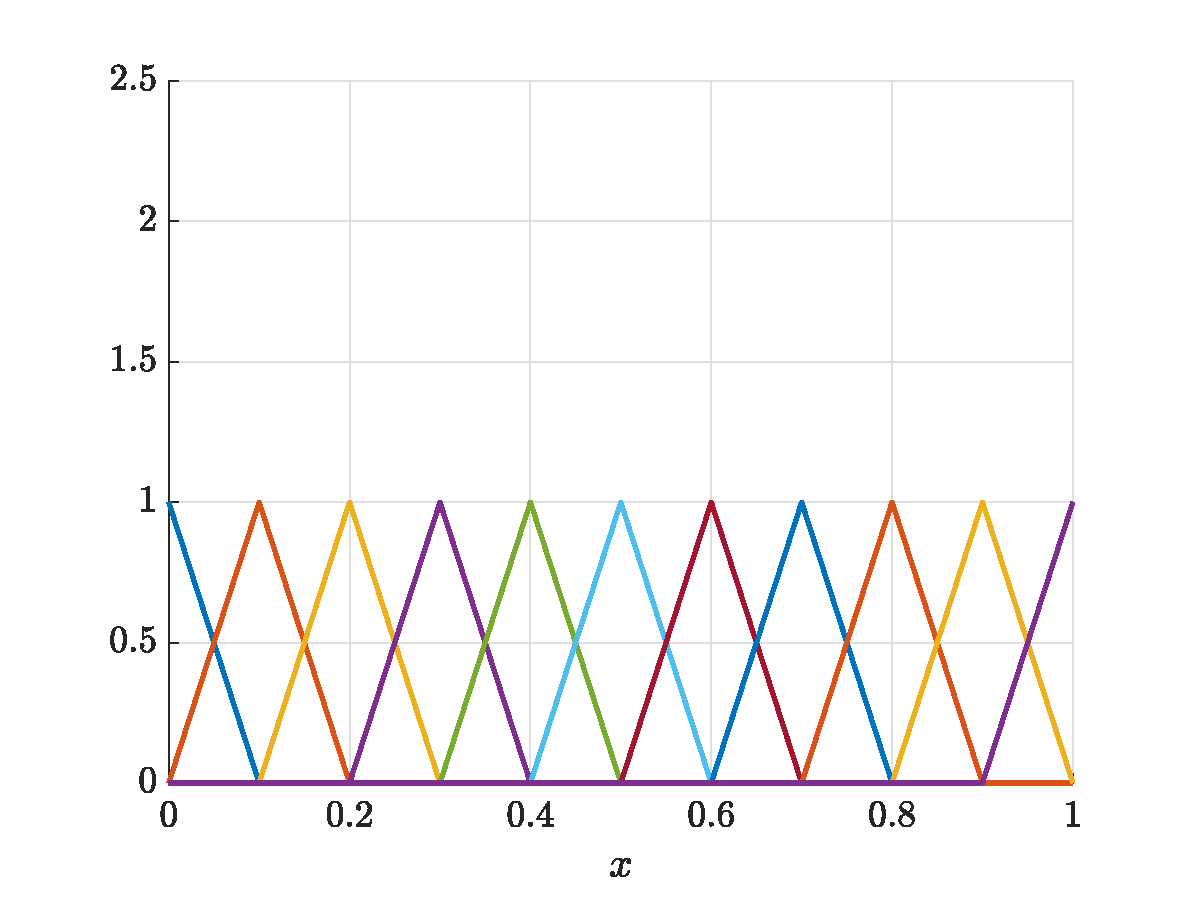
\includegraphics[width=0.45\textwidth]{./images/intro/hat}
	}
	\subfloat[RB basis functions\label{fig:ch1.1b}]{%
			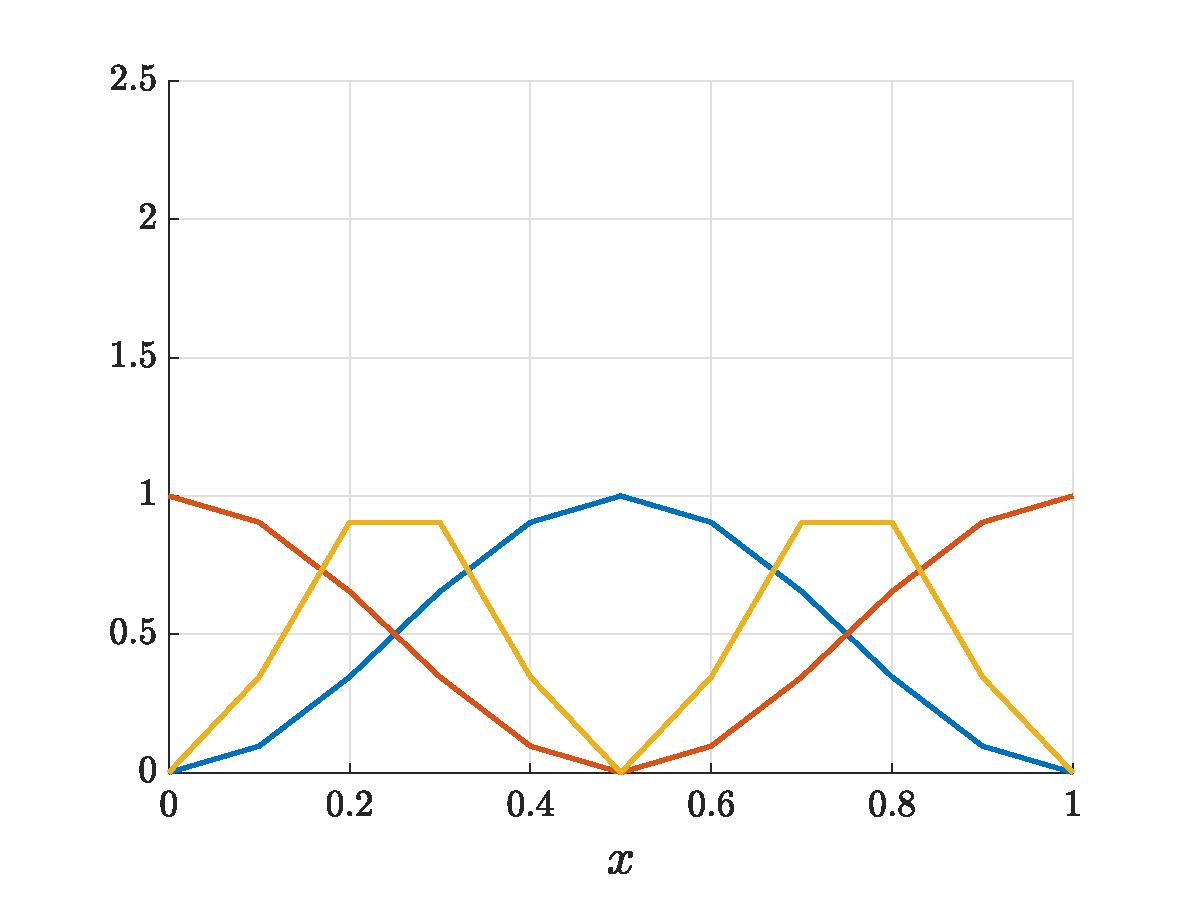
\includegraphics[width=0.45\textwidth]{./images/intro/pod}
	}
	\caption{spatial representation of MOR}
	\label{fig:ch1.1}
\end{figure}
where $\psi_i$ are chosen such that \eqref{eq:ch1.3} delivers comparable accuracy to \eqref{eq:ch1.2}. If $k \ll n$, we gain acceleration by evaluating only $k$ coefficients rather than $n$. Often, RB methods require the relation between $\psi_i$ and $\varphi_i$ to be a linear relation, i.e.
\begin{equation} \label{eq:ch1.3.1}
	\psi_i = \sum_{j=1}^n r_{ij} \varphi_j, \quad i=1,\dots,k.
\end{equation}
A rough sketch of basis functions $\varphi_i$ and $\psi_i$ is illustrated in \Cref{fig:ch1.1}. This is a \emph{spatial perspective} of reduced order modeling.

To be able to visualize the temporal aspect of MOR, we simplify \eqref{eq:ch1.1} to obtain an ordinary differential equation (ODE) $\ddot u(t) - u(t) = 0$, which can be expressed in terms of first order ODEs as
\begin{equation} \label{eq:ch1.4}
	\left\{
	\begin{aligned}
		\dot u(t) &= v(t), \\
		\dot v(t) &= -u(t).
	\end{aligned}
	\right.
\end{equation}
Introduction of the new variable $v$ is not only an algebraic tool, but carries a deeper insight into the dynamics of the original second order ODE. For instance, $H(u,v) = u^2 + v^2$ is a constant quantity, and can be interpreted as the energy of \eqref{eq:ch1.4}. Therefore, the value of $v$ is restricted by $H$ in a nonlinear sense. Another insight into the dynamics of \eqref{eq:ch1.4} is revealed when we consider vector fields in $(u,v)$ coordinate system, commonly referred to as the \emph{phase space}. \Cref{fig:ch1.2a} shows the vectors fields $\nabla H$ and $(\dot u, \dot v)^T$. We immediately notice the orthogonality of the two vector fields. Periodic behaviour of \eqref{eq:ch1.4} is a result of this delicate relation. Such properties of \eqref{eq:ch1.4} that are unchanged along a trajectories of \eqref{eq:ch1.4} are often referred to as \emph{symmetries} of \eqref{eq:ch1.4}.
\begin{figure} [t]
	\begin{centering}
	\subfloat[original vector fields\label{fig:ch1.2a}]{%
		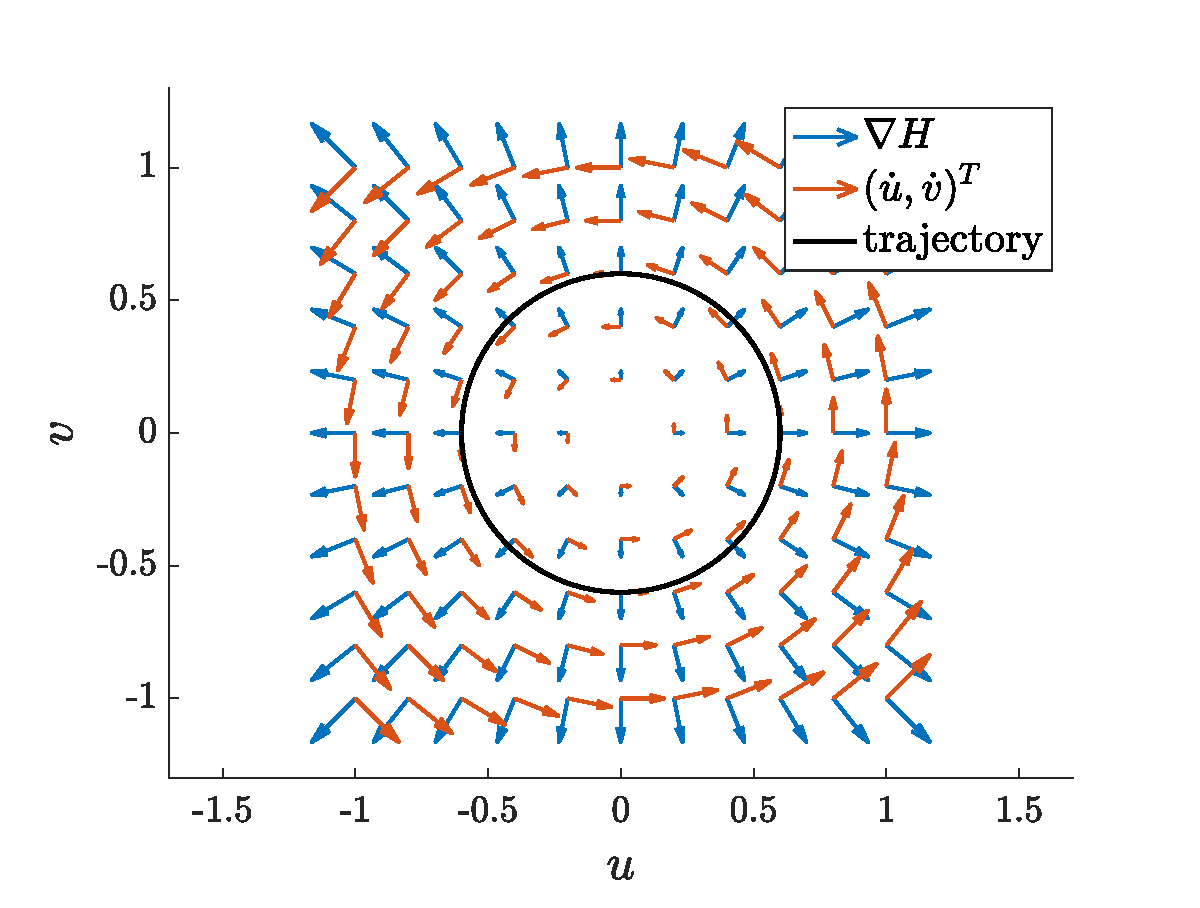
\includegraphics[width=0.45\textwidth]{./images/intro/orig}
	}
	\subfloat[transformation of vector fields\label{fig:ch1.2b}]{%
			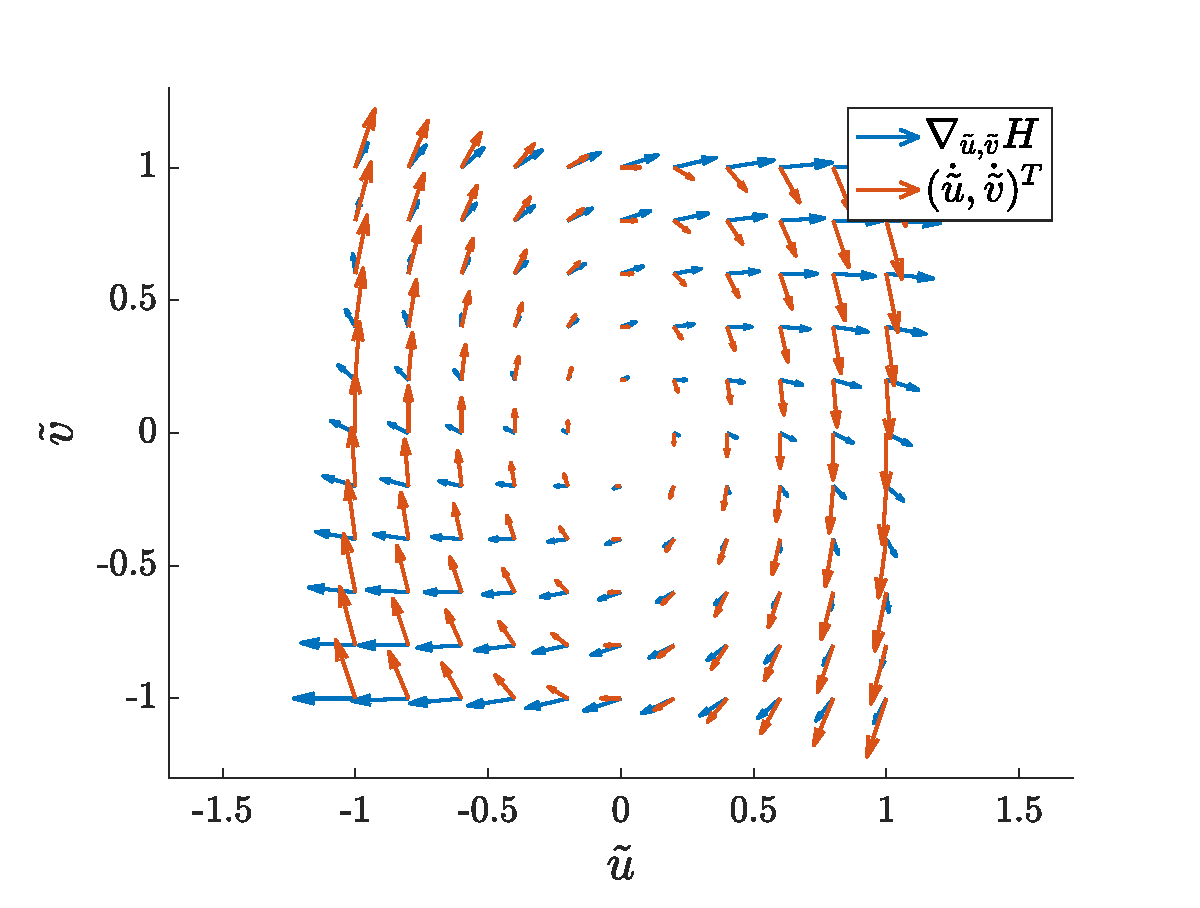
\includegraphics[width=0.45\textwidth]{./images/intro/trans}
	} \\
	\subfloat[symplectic transformation of vector fields\label{fig:ch1.2c}]{%
			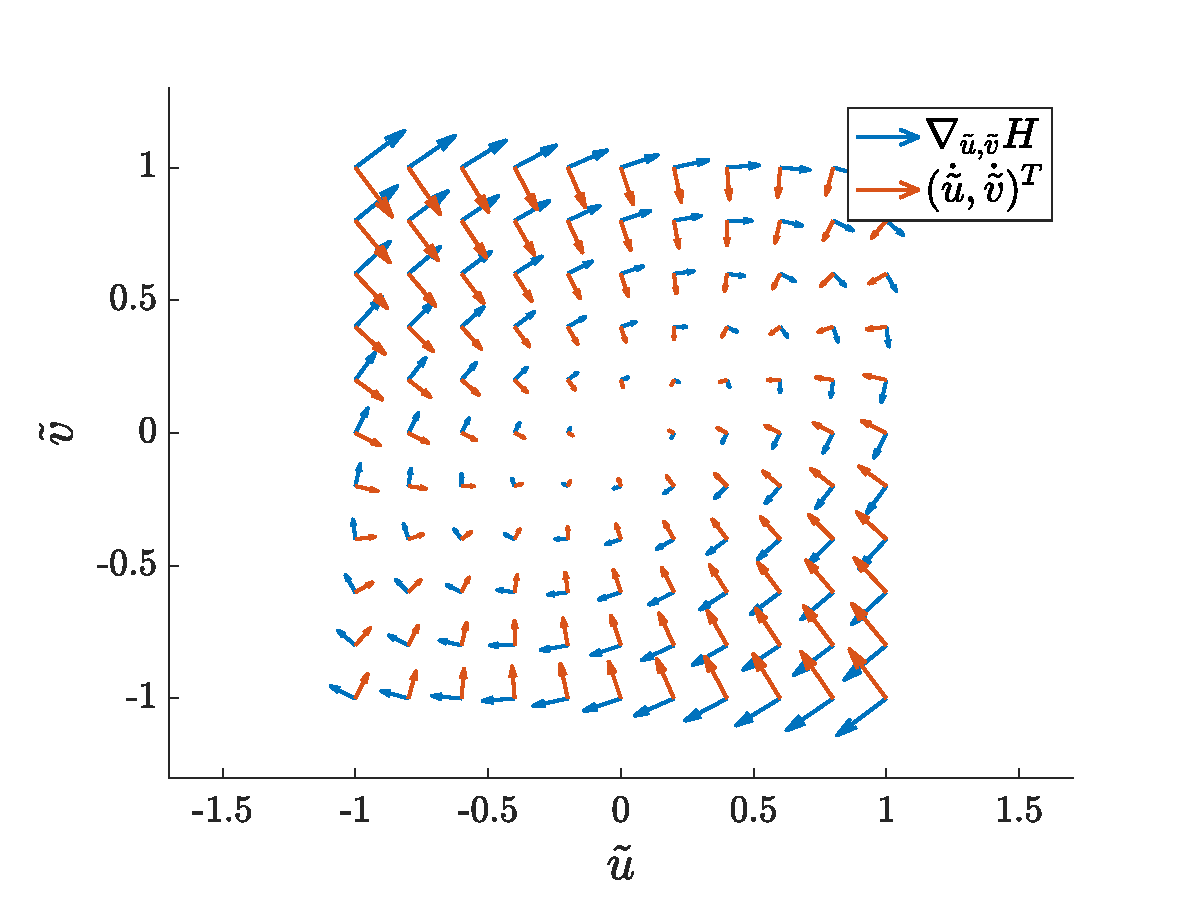
\includegraphics[width=0.45\textwidth]{./images/intro/symp}
	}
	\caption{temporal representation of MOR}
	\label{fig:ch1.2}
	\end{centering}
\end{figure}


Let us now study the symmetries of \eqref{eq:ch1.4} in a transformed coordinate system. \Cref{fig:ch1.2b} shows the transformation of $\nabla H$ and $(\dot u, \dot v)^T$ over some linear transformation $(\tilde u, \tilde v) = T(u,v)$. We notice that the orthogonality of the two vector fields is destroyed. Although, the dynamics of the original and the transformed system are the same, the transformed system carries less symmetry. For some class of linear transformations, \emph{symplectic transformations}, the orthogonality of the two vector fields is preserved. This can be seen in \Cref{fig:ch1.2c} where a linear symplectic transformation is applied to $\nabla H$ and $(\dot u, \dot v)^T$.

In a numerical approximation, loss of symmetries can have profound consequences for the overall dynamics of a system. For example, the periodic trajectory of \eqref{eq:ch1.4}, which is a distinctive feature of the dynamics, may no longer remain periodic in a non-symmetric coordinate system.

In the context of MOR basis functions, e.g., those in \Cref{fig:ch1.1a}, can be viewed as a basis for the phase space. Subsequently, a solution expanded in this basis can be translated as a vector in the phase space. The relation \eqref{eq:ch1.3.1} is therefore interpreted as a change in the coordinate system. This is the \emph{temporal perspective} of MOR.  

Similar to \eqref{eq:ch1.4}, we can define orthogonal vectors fields for \eqref{eq:ch1.1} as $\nabla H$ and $(\partial u/\partial t,\partial v/\partial t)^T$ with $v = \partial u/\partial t$ and $H(u,v) = \int v^2 + (\partial u / \partial x)^2 \ dx$. Therefore, we expect a general RB method to result in a non-symmetric phase space. In particular since the patterns in the ensemble of solutions to \eqref{eq:ch1.1} does not reveal the subtle relation between the two vector fields.

Nonlinear invariants and symmetries, such as those discussed above, are a fundamental feature of hyperbolic system of PDEs. Loss of symmetries in such systems can help explain challenges in MOR of hyperbolic problems.

The main aim of this thesis is to seek RB techniques that construct a reduced phase space that captures the symmetries of the high-fidelity system of PDEs. This ensures conservation of some nonlinear invariants and, subsequently, a good approximation of the overall dynamics in the reduced system. Hamiltonian systems, as systems that are driven by symmetries, are studied intensively from MOR view point. We then develop methods that preserve symmetries of a fluid flow.

\section{Overview of The Thesis}
The overall goal of this thesis is to study and develop RB techniques that preserve nonlinear invariants, symmetries, and conservation laws. Furthermore, it aims to understand the stability and robustness properties of these methods, compared to conventional RB techniques. This thesis mainly focuses on the MOR of time-dependent and, in particular, hyperbolic PDEs. A particular emphasis is put on model order reduction of Hamiltonian systems to understand the role of time in structure-preserving MOR. The main results are then generalized to construct MOR methods for fluid flow.

\Cref{chapter:2} surveys the background on smooth manifolds and Hamiltonian systems. We introduce the concept of geometric symmetry and how it relates to the dynamics of a time-dependent differential equations. We also briefly introduce methods for conserving these symmetries in a numerical evaluation.

An overview of the theory of model order reduction is presented in \Cref{chapter:3}. We present conventional RB techniques, e.g. proper orthogonal decomposition and the greedy method, for generating an accurate reduced basis. Galerkin and Petrov-Galerkin projection is then discussed to construct a reduced system. This chapter discusses the efficient evaluation of nonlinear terms by introducing the empirical interpolation method.

Symplectic MOR for Hamiltonian systems is developed in \Cref{chapter:4}. It is discussed how symplectic transformations can be used to construct a reduced Hamiltonian system that preserves the dynamics of the high-fidelity Hamiltonian system. We present a greedy method for the generation of a symplectic basis as well as other SVD-based symplectic model reduction techniques. Accuracy, stability, and efficiency of the method are discussed and illustrated by numerical experiments.

In \Cref{chapter:5} we couple the symplectic model order reduction with a weighted inner-product. We show that this can be viewed as a natural generalization of the symplectic MOR. Numerical experiments are presented to illustrate how this method can be beneficial when an unstructured numerical discretization is used in the high-fidelity system.

\Cref{chapter:6} presents symplectic MOR in the context of dissipative Hamiltonian system. It is discussed how a canonical extension of the dissipative Hamiltonian system yields a closed and conservative system. An application of a symplectic MOR on an extended system can help with a correct evolution of the Hamiltonian. The performance of this method is illustrated through simulations of dissipative Hamiltonian and port-Hamiltonian systems.

A conservative model reduction of fluid flow is presented \Cref{chapter:7}. It is explained how the skew-symmetry of differential operators in a fluid flow can help to recover the conservation of quadratic invariants, e.g., energy, at the level of reduced system. It is discussed how this gives rise to a physically meaningful reduced system with quadratic invariants with respect to the reduced variables. Stability properties of the method is illustrated through various numerical experiments of incompressible and compressible fluids.
